\documentclass[12pt, letterpaper]{article}\usepackage[]{graphicx}\usepackage[]{color}
% maxwidth is the original width if it is less than linewidth
% otherwise use linewidth (to make sure the graphics do not exceed the margin)
\makeatletter
\def\maxwidth{ %
  \ifdim\Gin@nat@width>\linewidth
    \linewidth
  \else
    \Gin@nat@width
  \fi
}
\makeatother

\definecolor{fgcolor}{rgb}{0.345, 0.345, 0.345}
\newcommand{\hlnum}[1]{\textcolor[rgb]{0.686,0.059,0.569}{#1}}%
\newcommand{\hlstr}[1]{\textcolor[rgb]{0.192,0.494,0.8}{#1}}%
\newcommand{\hlcom}[1]{\textcolor[rgb]{0.678,0.584,0.686}{\textit{#1}}}%
\newcommand{\hlopt}[1]{\textcolor[rgb]{0,0,0}{#1}}%
\newcommand{\hlstd}[1]{\textcolor[rgb]{0.345,0.345,0.345}{#1}}%
\newcommand{\hlkwa}[1]{\textcolor[rgb]{0.161,0.373,0.58}{\textbf{#1}}}%
\newcommand{\hlkwb}[1]{\textcolor[rgb]{0.69,0.353,0.396}{#1}}%
\newcommand{\hlkwc}[1]{\textcolor[rgb]{0.333,0.667,0.333}{#1}}%
\newcommand{\hlkwd}[1]{\textcolor[rgb]{0.737,0.353,0.396}{\textbf{#1}}}%
\let\hlipl\hlkwb

\usepackage{framed}
\makeatletter
\newenvironment{kframe}{%
 \def\at@end@of@kframe{}%
 \ifinner\ifhmode%
  \def\at@end@of@kframe{\end{minipage}}%
  \begin{minipage}{\columnwidth}%
 \fi\fi%
 \def\FrameCommand##1{\hskip\@totalleftmargin \hskip-\fboxsep
 \colorbox{shadecolor}{##1}\hskip-\fboxsep
     % There is no \\@totalrightmargin, so:
     \hskip-\linewidth \hskip-\@totalleftmargin \hskip\columnwidth}%
 \MakeFramed {\advance\hsize-\width
   \@totalleftmargin\z@ \linewidth\hsize
   \@setminipage}}%
 {\par\unskip\endMakeFramed%
 \at@end@of@kframe}
\makeatother

\definecolor{shadecolor}{rgb}{.97, .97, .97}
\definecolor{messagecolor}{rgb}{0, 0, 0}
\definecolor{warningcolor}{rgb}{1, 0, 1}
\definecolor{errorcolor}{rgb}{1, 0, 0}
\newenvironment{knitrout}{}{} % an empty environment to be redefined in TeX

\usepackage{alltt}
\usepackage[margin=1.5in]{geometry}
\usepackage{caption}
\usepackage{subcaption}
\usepackage{graphicx}
\usepackage{array}
\usepackage{longtable}
\usepackage{wrapfig}
\IfFileExists{upquote.sty}{\usepackage{upquote}}{}
\begin{document}

\tableofcontents
\newpage
\section*{Executive summary}

Past-sales analyses is an important source of information for manufacturing companies. The analysis of how sales evolved in the past provides evidence regarding the performance of products in the market, and the impact of the manufacturing and marketing strategies, adopted by the companies, on their sales and profit. Such evidence often takes the form of visual plots or financial indicators that help to quantify the performance of the business and support the management in taking decisions. Based on such analyses manufacturing companies can identify drawbacks in their strategies and try to improve them. The process of taking decisions about what plan of action to adopt in the future based on past data is rather empirical, because it is only based on evidence collected in the past and is lacking evidence about the future. In practice sales follow certain patterns that might be independent from the business plans and future sales most likely will not look like the past sales. Therefore one needs to take into consideration also the fact that the market is changing and be able to foresee how the sales will evolve independent from the present conditions and approaches of the business. Sales forecasts can provide information which is complementary to the past-sales data analyses, that can be used in order to identify intervention points and decide about what strategy would be best to adopt in the future.

In this study we will mainly focus on statistical methods that can be used to uncover and reproduce the mechanisms that affect the behavior of the sales. The first step in this direction is to visually look for the main patterns in the data set, and try to answer questions like: Is there a recurring pattern? Do the data follow a discernible trend in time or do they seem more or less random? One can already answer these questions with a graphical representation of the data set. Once the main patterns are identified, the second step is to try to reproduce them. For this purpose we will be looking for models that can best describe the data set and try to understand: Do the recent sales evolve independently from the past sales and give a certain pattern in time, or they depend on former sales points? And if they depend on former sales points is there a local mechanism which involves only a few data-points close to each observation which is responsible for the sales patterns? Or the sales values depend on both the recent and distant former sales with equal weights? These are questions that concern the mechanism that the model employs in order to reproduce the patterns. In this dissertation we work along these questions, try different methods and discuss how they affect the performance of the forecast.

\section{Introduction}

Sales data have the form of a time series. A time series is an object that describes the evolution of an observable quantity over time. It consists of a collection of observations made at discrete points in time and at equal time intervals. The time intervals can vary from seconds to quarters or even years, meaning that the size of the time series object can get arbitrarily large as we approach the continuous time. Time is directional and the time series inherits this property meaning that observations happen along the natural ordering of time. For example, if $t_2>t_1$, observations at time $t_2$ always happen at later times than the observations at time $t_1$. This property implies the existence of a causal relation between observations at later times and the past, i.e. $O(t_2) = O(t_2, O(t_1);t_2>t_1)$, the observation made at time $t_2$ has an implicit dependence on the observations made at previous times. 

Time series forecasting is the process of predicting the values of a time series object in time based on its values in the past. One needs to first model the past time series and then use this model to obtain a forecast. If the model is constructed in a way that reproduces as much as possible the patterns observed in the former data, the forecast will also have these characteristics because it is using the mechanism of the model. Such a model needs also to preserve certain properties of a time series, such as to generate values that follow the natural direction of time and to preserve the causality. In a system that is not causal predictions can be fixed to the observations in all boundaries and a subset formed by a random selection of observations preserves the mechanisms of the system. This allows for more flexibility and more information to obtain predictions. In a time series however we need to preserve the ordering and continuity in time when performing predictions or forming subsets. This leaves the predictions unbounded in the upper limit and therefore there is less information available for determining the forecast. Naturally one can expect that it is challenging to obtain a forecast of high accuracy. 

In the following sections we will introduce the basic concepts and the main challenges of sales forecasting. Then we will use an artificial data set that simulates the sales of a single product and apply models that use different mechanisms for detecting and reproducing patterns. We will further apply the most promising methods on a realistic data set and discuss their performance. At the end we will present our final conclusions and suggest possible ways to improve. 

\section{Problem description}
In this study, we are interested in forecasting time series of weekly sales data. The length of the forecasting horizon considered throughout this study is one year. The first challenge that we face is to select a model that captures the principal mechanisms of a time series. Typically there are two main patterns that such a model should be able to describe:
\begin{itemize}
\item The trend of the sales. This gives the long-term evolution of the sales as a function of time. This component is often varying slowly with time. Except from the tendency to buy or not a specific product, it also includes the effects of other variables such as the evolution of the price over time.
\item The seasonal component. This component is given by a periodic function of time, which describes the patterns that are repeating over consecutive periods. It is responsible for the fast variations with respect to time within a period. Throughout the study we will discuss cases that show a yearly seasonality.
\end{itemize}
In practice it is not always straightforward to extract the seasonal pattern from a time series. For instance the time series can show a weak pattern but still important and therefore not easy to identify. Or the seasonal pattern can be also changing in time. In the following section we are going to discuss different approaches for capturing these mechanisms.

It is not only the selection of the model that it is challenging, but also to construct a model that learns in a way that it preserves the characteristics of a time series as were introduced earlier. Usually these properties are embedded either in the way that the model learns from previous values, or in the process that is used for determining the model. They are either intrinsic properties of the model we use, or embedded in a process, like the cross-validation.  

Another major challenge that we face is to estimate the accuracy of the forecast. In order to estimate the accuracy of the forecast from a prediction error, we need to allocate a part of the data set for performing the prediction and evaluate the error with respect to the actual observations. This part of the data set usually contains the most recent observations and its size needs to be comparable to the length of the period that we typically forecast. This also means that any patterns hidden in these observations (like a sudden change in the trend or a flattening of the trend) will not contribute to the mechanism of the model. In this sense the forecasts calculated from such a model can be outdated and whenever possible, we should try to use as much of the information disclosed by the data set as possible for determining the models, but still be able to estimate the prediction error of the method. 

Finally another challenge that we face is the size of the data set. Time series with weekly sales are not large but usually a data set can contain multiple time series, for which we need to evaluate forecasts. It can be a challenging task to produce forecasts for each individual time series object in a large data set, firstly because it gets computationally expensive and secondly because it might be the case that we will not be able to describe all the time series with the same method. 

\section{Methodology and results}

In this section we will apply different methods for sales forecasting and discuss their performance. We divide the methods in two main categories, methods that do not model the seasonal component but focus on the trend, and methods that model both seasonal and trend components. The models are based mainly on statistical and regression methods.

We will start with a brief introduction of each of the methods, followed by a discussion of the application and the performance of the different methods on an artificial data set that simulates a time series of sales. We used an artificial data set for two reasons: In first place in order to avoid discussing extensively the data sets of the company; And the second reason is to benchmark the performance of the different methods against an ideal data set whose behavior and properties are fully determined. We embed in the artificial data set certain seasonal and trend patterns, as well as the dependence on other variables so that the actual values of the target variable are known for the periods we want to forecast. This way we get an idea of how well the different methods perform compared to the actual behavior. An artificial data set does not need data pre-processing as opposed to a real data set. We will apply the most promising methods on a realistic data set. In the realistic data set we will discuss the pre-processing steps and the performance of the different methods in forecasting cases that show different sales patterns. We will conclude this section with a brief discussion on the computational efficiency of the different methods.

To measure the performance of a model we rely on three different errors. The fitting error, which measures how far the target values are from the actual observations. The prediction error, which measures how far the predicted values are from the actual observations. And the cross-validation error, which measures how well a model generalizes to the full data set. As a metric for the errors we are using the Root Mean Square Error (RMSE), because it has the same order of magnitude as the observations in the data set and we can compare its values across different methods. To compare among different data sets we use the standardized RMSE, which is the RMSE of the data set divided with the standard deviation. 

In the cross-validation process we repeatedly split the full data set into two subsets, one used for training a model and the other one for the calculation of a prediction error (testing), while we vary the size of the subsets in each step. Since we are working with time series objects we need to split in ways where the testing set is always at later times than the training set. In order to do this we adopt an expanding window for the training set. In each step of the cross-validation process the training window expands by one observation. The initial window includes the first year of observations and the length of the forecasting horizon used for the evaluation of the prediction errors is always one year, similar to the forecasting horizon of the actual forecast. This way of evaluating the cross-validation error measures how well the model generalizes when the training set grows in size. This error gives an idea of how well the model would perform if we used it for obtaining forecasts in the future as the data set grows in size. A way to embed some of the properties of the time series to the mechanism of a regression model is to employ this process of cross-validation for the selection of the regression model (i.e. the degree of a polynomial), because when selecting the model that minimizes the cross-validation error, it imposes the condition that predictions can only get based on past-data.

To model the data set we adopt the following methodology. In order to evaluate the model coefficients, we use all years except the last one and follow approaches which select those values of the coefficients that minimize the square of distance from the actual values. The last year of the data set is used for the calculation of the prediction error. For the evaluation of the model hyperparameters, like smoothing parameters or order parameters we select the value of the hyperparameters that either minimize the cross-validation error or maximize an information criterion. 

\subsection{The artificial data set}

\begin{figure}[h!]
\centering
\begin{subfigure}{0.9\textwidth}
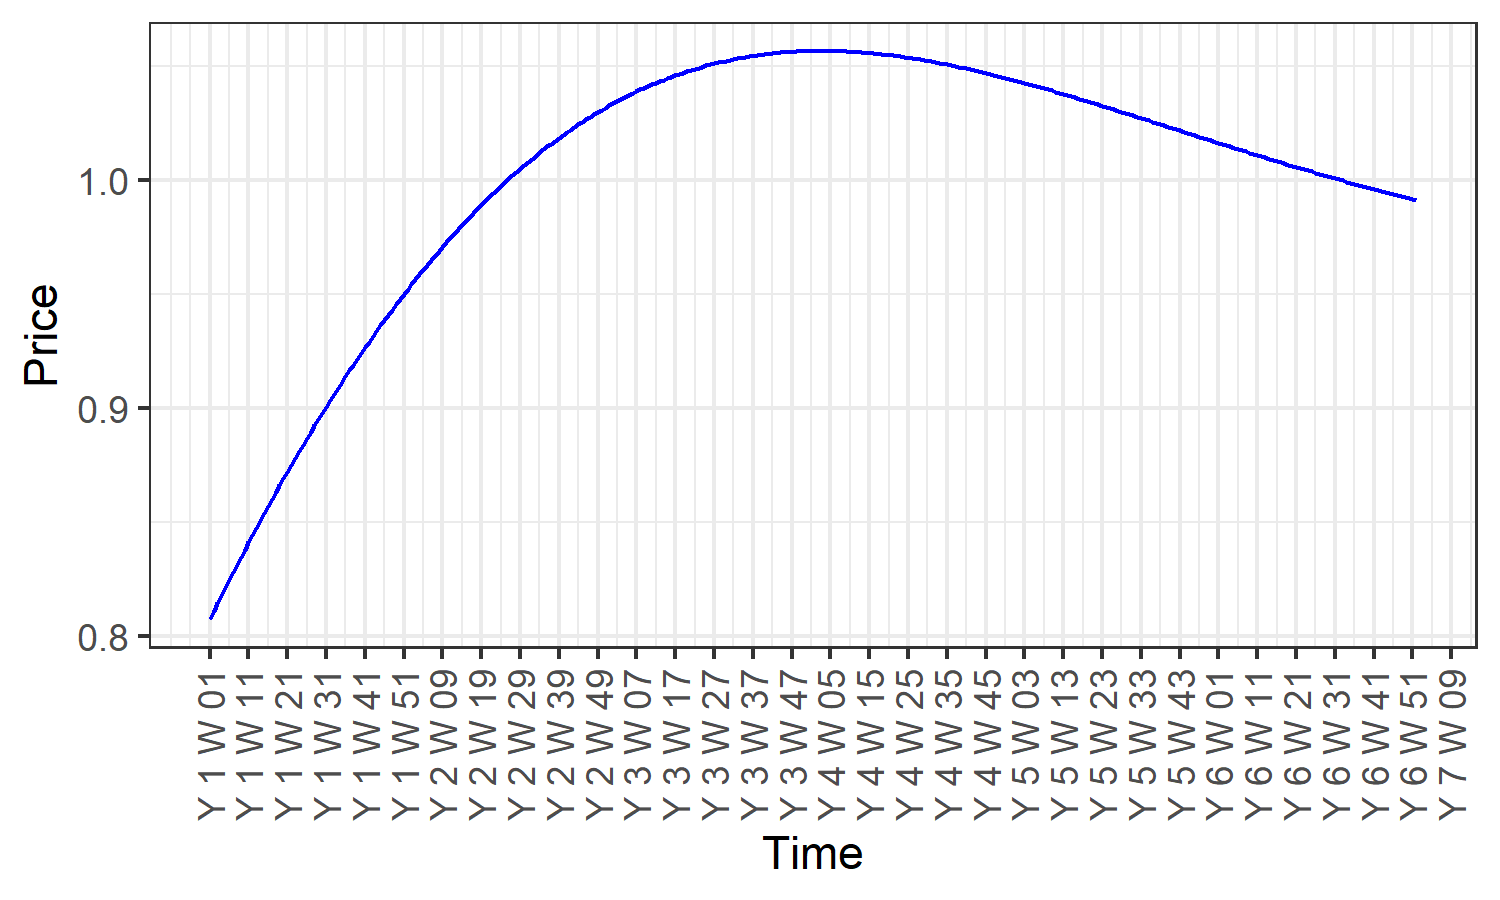
\includegraphics[trim = {0 0 0 0}, width = \textwidth]{"figures/price.png"}
\end{subfigure}
\hfill
\begin{subfigure}{0.9\textwidth}
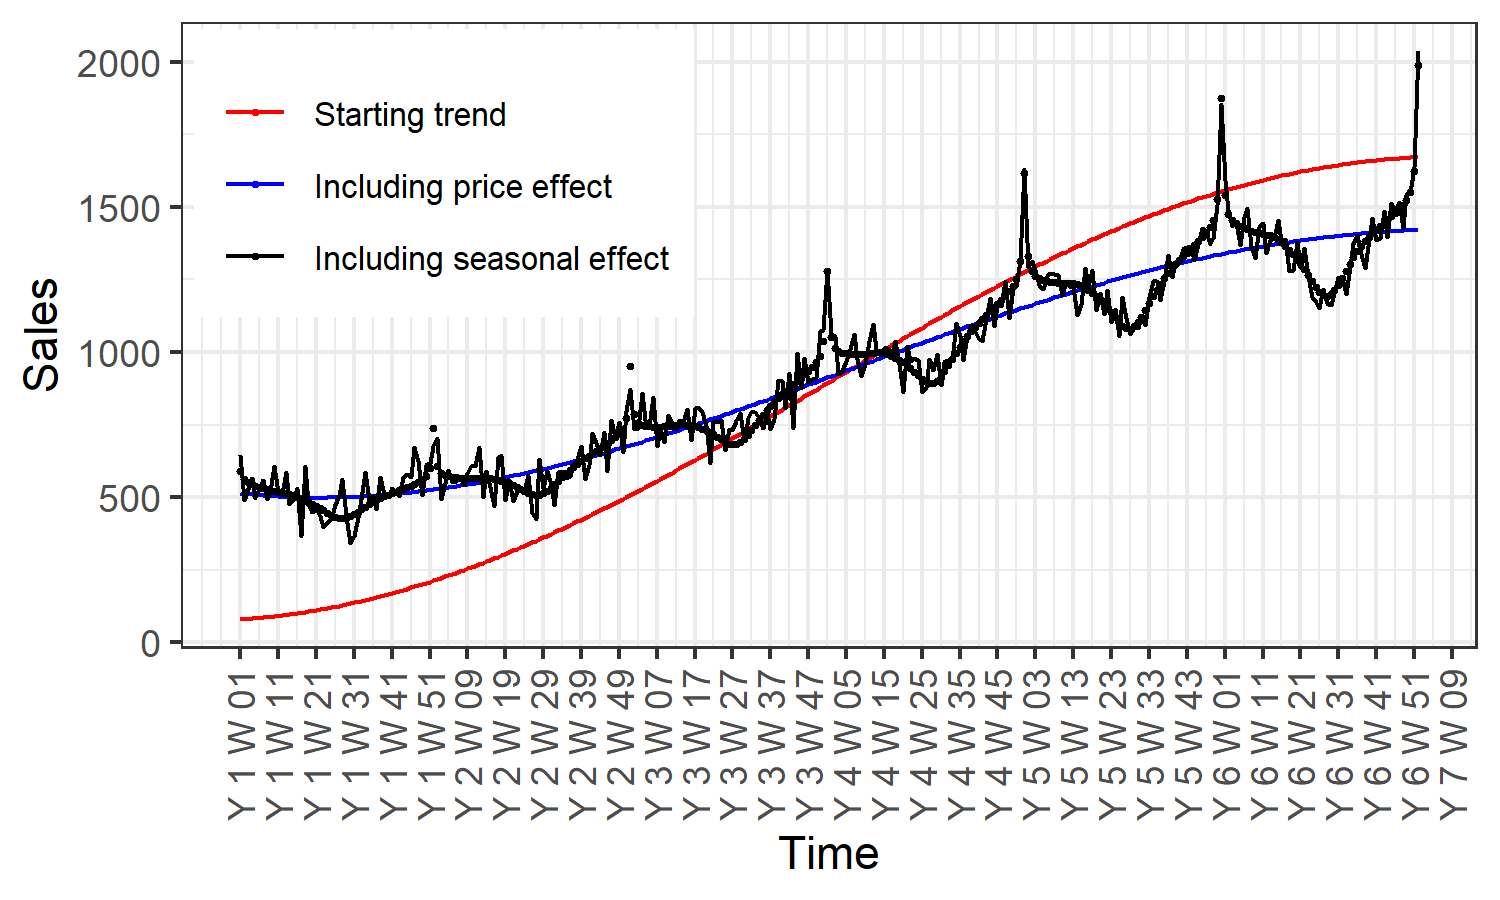
\includegraphics[width = \textwidth]{"figures/sales_model.png"}
\end{subfigure}
\caption{The different contributions to the sales on the artificial data set.}
\label{fig:model_data}
\end{figure}

Let us briefly introduce the artificial data set. The artificial data set is constructed in a way that it preserves certain characteristics of a real data set, such as the weekly data points, the yearly periodicity and 6 years of data availability. The different contributions to the sales are given by an equation of the form
\begin{equation}
F(t) = T(t) + \frac{a}{P(t)} + S(t) + \epsilon(t) , 
\label{eq:data_model}
\end{equation}
where the sales ($F$), take contributions from the trend ($T$), are inversely proportional to the price ($P$), $S$ is the seasonal component and $\epsilon$ is the noise responsible for small-scale variations.
In fig.\ref{fig:model_data} we reveal the effects of the different contributions to the sales. There is a tendency of increasing sales over time (red line). Under the assumption that the price has a negative effect on the sales, the increasing price is leveling off the increase in the trend of the sales and gives the blue line. We also include the seasonal pattern and obtain the black line. The seasonal pattern imposes a tendency to have more sales during the winter period and at the end of the year, while the sales decrease over the summer period.   

\subsection{Seasonal naive and drift models}

\begin{figure}[h!]
\centering
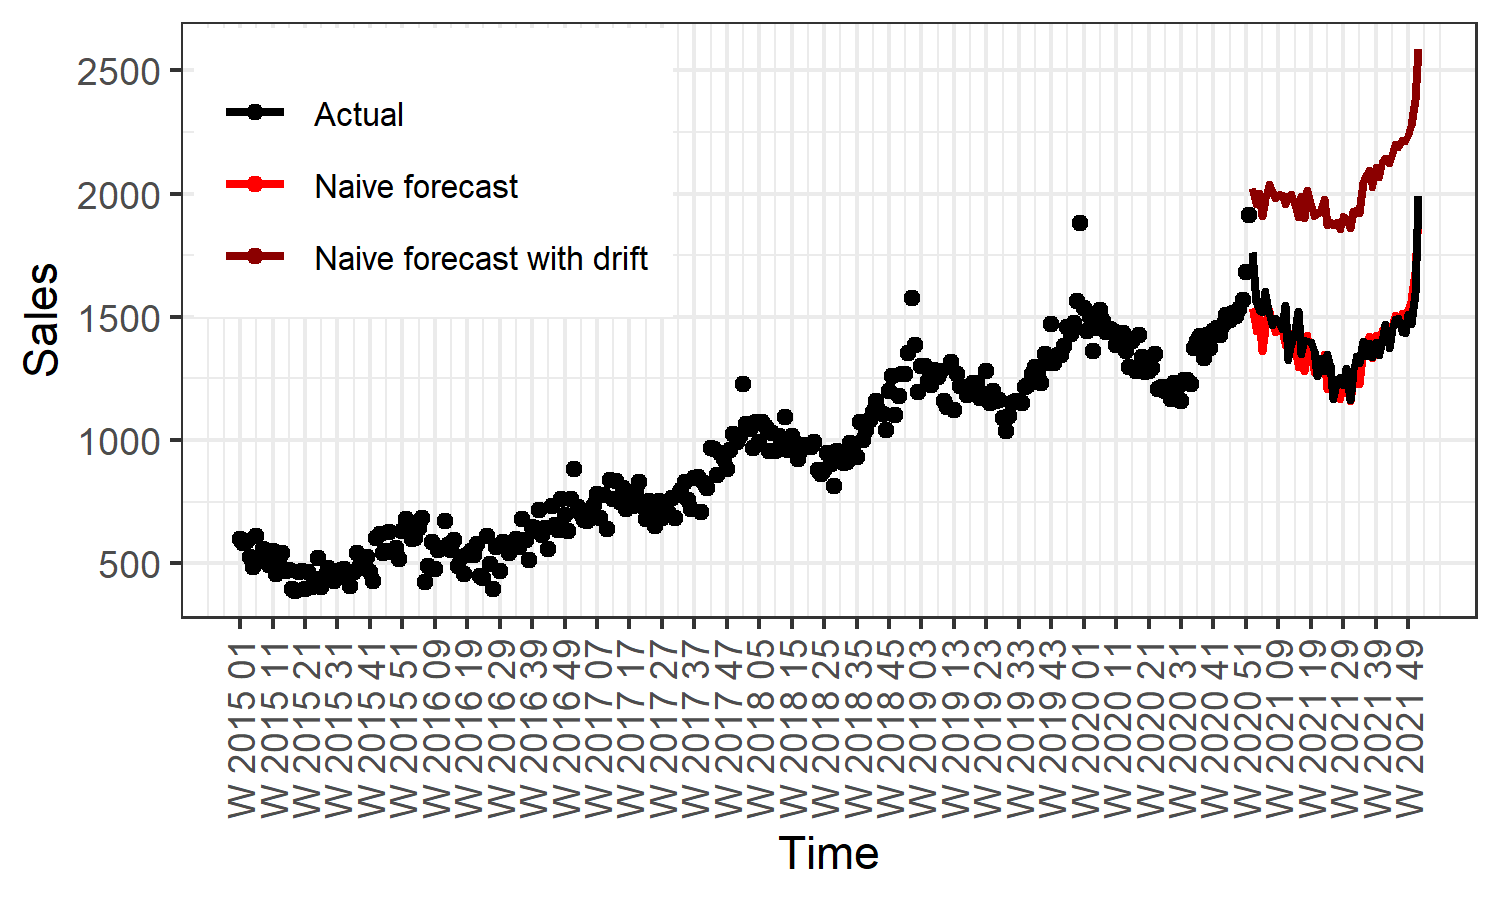
\includegraphics[width = 0.9\textwidth]{"figures/naive.png"}
\caption{Comparison of forecasts between the seasonal naive and drift methods.}
\label{fig:naive}
\end{figure}

A simple approach to the sales forecasting is to reproduce patterns in the data set under the assumption that they do not change with time. For example repeating the last year's sales unchanged (naive method) will work for a case where the trend is no longer changing. To account for changes in the trend, a seasonal naive approach can be combined with a drift term\cite{Hyndman_book}. We compare the two methods in fig.\ref{fig:naive}. The forecast from the seasonal naive method (light red line) performs quite well, since the time series tends to stabilize. The forecast obtained from the drift term (dark red line) is influenced by the peak of the seasonal period where the time series terminate. This issue would have been avoided if the seasonal pattern was extracted from the time series and the drift term was calculated only from the trend component. Decomposition methods are good candidates for this purpose. In tab.\ref{tab:Comparison} we look at the errors of the two different methods. The fitting error for the seasonal naive method is large because the truncation of the time series cannot fit well the early part of the time series. Only if the time series was a straight line, the fitting error would be zero. The drift term dramatically improves the fitting error, but it leads to a much larger prediction error due to the high impact from the seasonal peak. 

\subsection{A seasonal toy-model for yearly sales forecasting}

\begin{figure}[hb!]
\centering
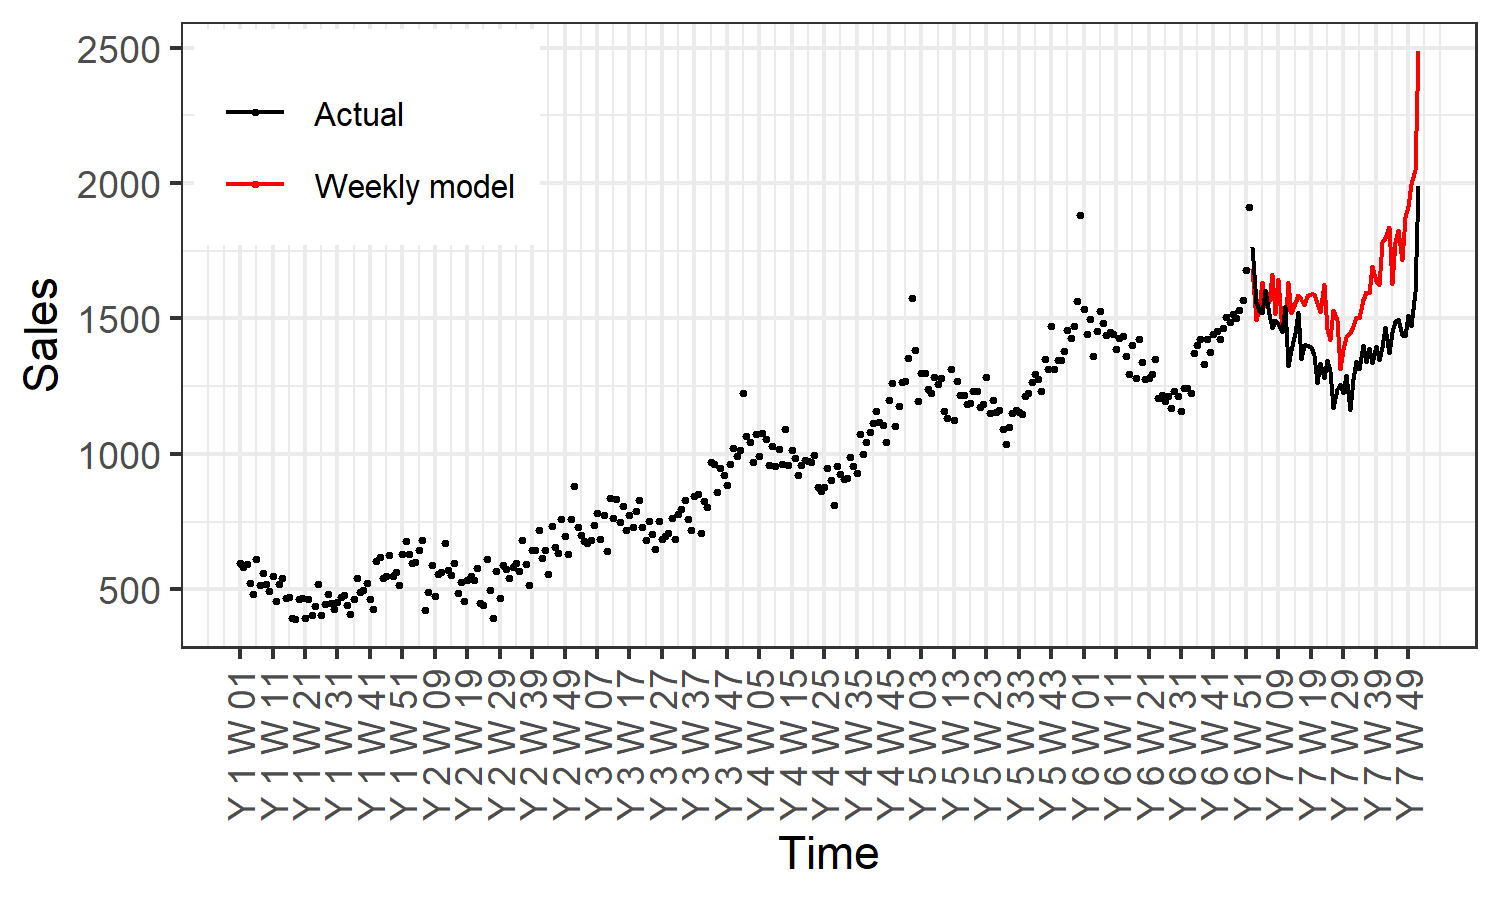
\includegraphics[width = 0.9\textwidth]{"figures/linear_model.png"}
\caption{Forecast obtained from a yearly regression toy-model.}
\label{fig:linear_model}
\end{figure}

Here follows a brief discussion of a simple toy model that we propose and which assigns to each week of the year a different linear trend. The sales of each week as a linear function of the year are given by
\begin{equation}
F_w(Y) = \alpha_w*Y+\beta_w ,
\end{equation}
where $Y$ stands for the year and $w$ is an index that runs over the weeks of a year. Taking the values of the parameters $\alpha_w$ and $\beta_w$ from linear regression, the model can predict the sales for new years. The data set is divided in multiple independent data sets, each one giving the yearly evolution of sales for a given week. This leaves each subset with only a few points to model, but one can always fit a line. Splitting between a training and a test set requires at least two points for training the model and one point for testing. A data set of at least three years allows to calculate both the fitting and prediction errors. We calculate an error for each weekly subset. We evaluate the final model error averaging over the RMSE of each week. 
% I calculated the error over all 52 weeks.

In fig.\ref{fig:linear_model} we see that this model captures the seasonal behavior but still deviates from the actual values. This model estimates the trend of each week accounting for the year-to-year evolution. Indeed this is a seasonal model that is missing completely any effects that come from the variations of the trend happening within a year. Moving averages and autoregressive models are indeed different approaches that model each value of the target taking into account also the values of neighboring weeks. 

\subsection{Forecasts using the seasonal naive method}

In a time series there are two main patterns, the seasonal pattern and a (long-term) trend. A reliable forecast would need to be able to extract and reproduce both of them. Trying to model the time series as a whole can lead to failures like the drift term applied on the full time series getting a strong influence from a seasonal peak in fig.\ref{fig:naive}. To avoid such cases one can first decompose the time series into its components using classical decomposition\cite{Hyndman_book} or Seasonal and Trend decomposition using Loess (STL)\cite{STL}. Here we combine the classical and STL decompositions with different techniques for forecasting the trend component. For forecasting the seasonal component we use the seasonal naive method.

Classical decomposition is based on smoothing with moving averages, while STL is using local regression smoothing for the trend and seasonal components. In tab.\ref{tab:Comparison}, we see that the STL decomposition error is smaller than the classical decomposition error. 

In fig.\ref{fig:cl_decomposition} we compare between linear (LR) and non-linear regression (NLR) for the trend component from the classical decomposition. The forecasts extend over 1,5 years instead of one year, because in the classical decomposition the trend requires half a year of observations ahead and for the last half year future observations are not available since the series terminates. Linear regression (red line) assumes that sales is a linear function of time. This is an improvement compared to the drift term since the slope is taken only from the trend and is chosen in a way that is minimizing the distance from the values of the target variable. Non-linear regression (blue line) assumes that the trend is a function of two variables, the price and time, given by a polynomial. Here we try two possible variables, one is the price (positive orders) and the other one is the $\frac{1}{Price}$ (negative orders). This way non-linear effects arise not only from the explicit dependence in time, but also from the price in an implicit way, since it is in general also a non-linear function of time. 
\begin{wrapfigure}{r}{0.5\textwidth}
\centering
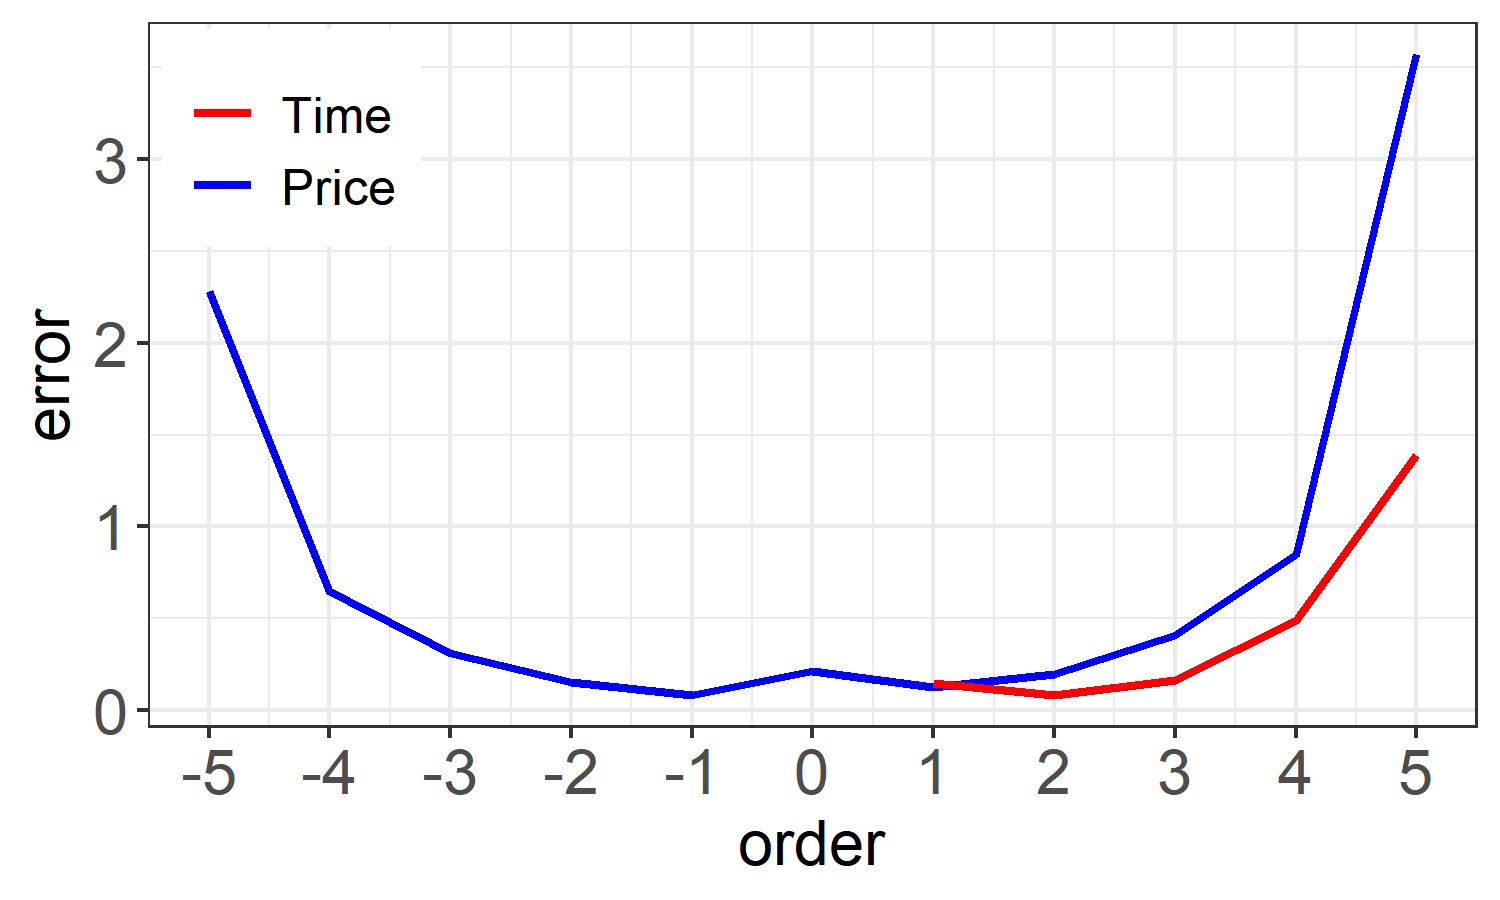
\includegraphics[width = 0.49\textwidth]{"figures/CV_error_nl.png"}
\caption{Cross-validation error as a function of the order for the price and the time variables.}
\label{fig:CV_error_nl}
\end{wrapfigure}
In fig.\ref{fig:CV_error_nl} we see that a linear dependence in $\frac{1}{Price}$ and a second order in time minimize the cross-validation error. In order to obtain the forecasts, the price is taken as constant and equal to the value of the last observation in the data set. In tab.\ref{tab:Comparison} is shown that the non-linear regression improves all fitting, prediction and cross-validation errors. 

\begin{figure}[h!]
\centering
\begin{subfigure}{0.9\textwidth}
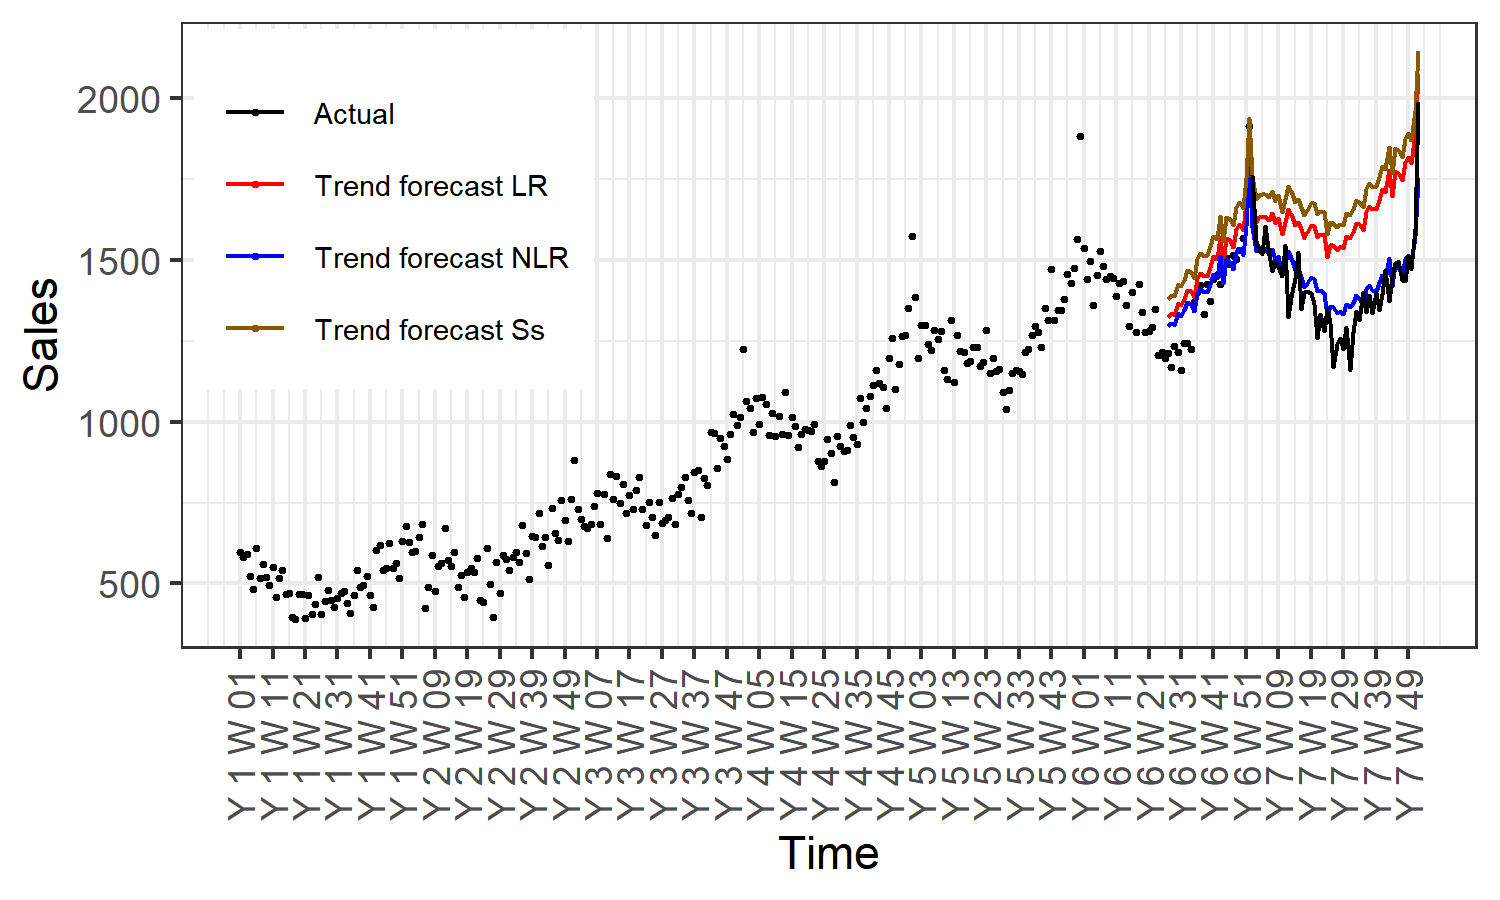
\includegraphics[width = \textwidth]{"figures/cl_decomposition.png"}
\caption{Classical decomposition}
\label{fig:cl_decomposition}
\end{subfigure}
\hfill
\begin{subfigure}{0.9\textwidth}
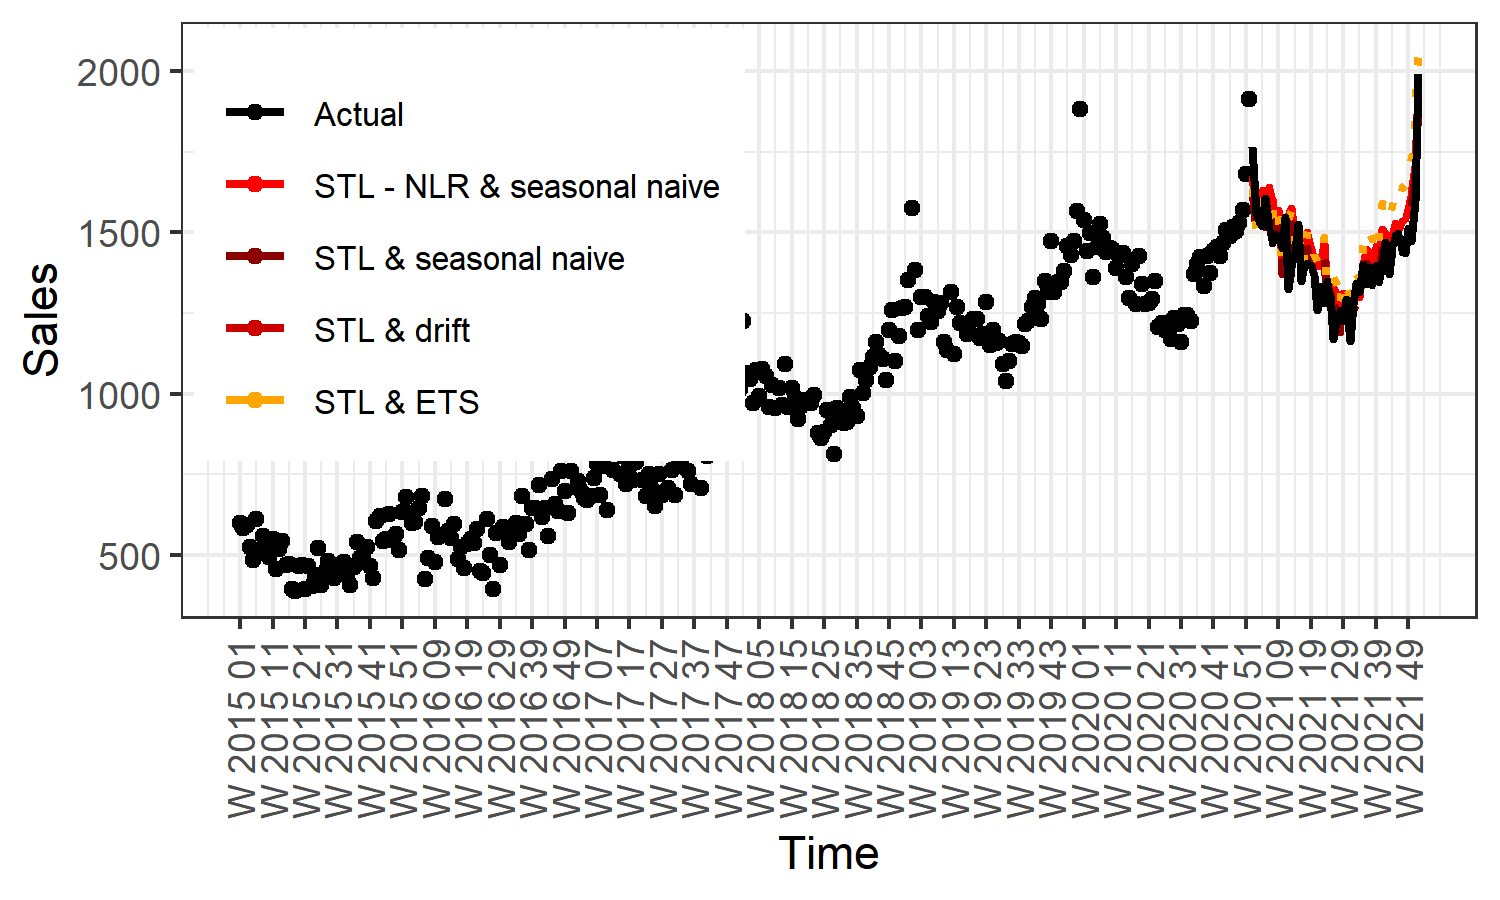
\includegraphics[width = \textwidth]{"figures/stl_decomposition.png"}
\caption{STL decomposition}
\label{fig:stl_decomposition}
\end{subfigure}
\caption{Comparison of decomposition methods used for seasonal naive forecasts that are combined with different models for trend forecasting.}
\label{fig:decomposition_models}
\end{figure}
In general increasing the degree of the polynomial can minimize the bias by reproducing local characteristics but will also increase the variance and possibly overfit. This makes the polynomials prone to divergences outside the fitting region. Piece-wise polynomials on the contrary rely on fitting different polynomials in different regions of the data set which contribute to the forecasts through the condition of continuity \cite{Statistical_Learning, Smoothing_Splines}. These functions are called splines. These functions when we include a smoothing term to the least squares method, decrease the variance. The smoothing term is switched on with a smoothing parameter. When its values are close to zero, a detailed fitting is done, otherwise strong variations are smoothed out. Here, even though the polynomials perform well, we also tried the regression with smoothing splines which could be useful in a realistic case. In this method we need to choose the order of the smoothing parameter for each of the variables used. For those variables that are varying slowly with time, a few degrees of freedom will suffice to describe the target, so we expect a larger value of the smoothing parameter. This is the case of the price variable which is varying slowly with time. On the contrary we want to obtain a dependence on time which is as detailed as possible, and therefore for time we take a value of the smoothing parameter that is small. In fig.\ref{fig:cl_decomposition} the dark orange curve corresponds to a smoothing spline with large smoothing for the price and negligible smoothing in time. Since the effects of the price are smoothed out the resulting forecast is similar to a linear function of time (red curve). In tab.\ref{tab:Comparison} we see that compared to the linear regression, the smoothing splines improve the fitting and cross-validation errors, but aggravate the prediction error, indicating possibly that they cannot capture the behavior towards the end of the time series.

In fig.\ref{fig:stl_decomposition} we combine the STL decomposition with different methods for modeling and forecasting the trend. A naive method for the trend (green line) performs very well, as expected since the series tends to stabilize. STL with a drift (purple line) improves compared to fig.\ref{fig:naive} dark-red line, since the drift term is calculated from the seasonally adjusted series (after removing the seasonal component). STL with exponential smoothing (ETS)\cite{Hyndman_book} for the trend performs also quite well but it can be seen in tab.\ref{tab:Comparison} that it gives a larger prediction error. Even though the STL with the naive method has the smallest prediction error, it has the largest cross-validation error. This means that it performs well in the last year of observations and grasps the mechanism in that region but does not generalize well to the full data set, so it is not reliable for future forecasts. On the contrary the drift and ETS methods have cross-validation errors that are close to the prediction errors  and therefore are more reliable for forecasting. ETS gives a lower fitting error compared to the naive and drift methods. Looking at the performance of the non-linear regression for the trend (STL-NLR), the trend fitting error is small compared to the decomposition error. Adding up for NLR-STL the prediction or cross-validation errors to the decomposition error, one can obtain an upper bound for the combined error. Doing this, we see that the resulting errors are similar to the errors of the other methods we combined with STL. 

\subsection{Forecasts beyond the seasonal naive method}

Until now the main focus has been to capture the mechanism of the trend component for the forecasts while the seasonal component has been treated with the seasonal naive method. Here we will discuss two methods that are modeling the mechanism of the seasonal component as well, the Holt-Winters \cite{Winters,Holt} and the AutoRegressive Integrated Moving Average (ARIMA) \cite{ARIMA}.

The Holt-Winters' method is introducing a smoothing parameter for the seasonal component which allows for the more recent seasonal observations to contribute with higher weights. We evaluate the model parameters on the training set and perform cross-validation. Keeping the same parameters, we apply the Holt-Winters' model on the full data set and calculate the forecast. Looking at fig.\ref{fig:hw_stl}, we see that the Holt-Winters (green line) leads to forecasts that are not very different from the ETS for the trend (blue line), where the smoothing parameter was introduced for the trend but the seasonal component was taken unchanged from the last year of observations. Comparing the errors in tab.\ref{tab:Comparison} we observe that even though the fitting and prediction errors are larger than STL combined with ETS, the cross-validation error is smaller meaning that it generalizes better over the data set.
\begin{figure}[h!]
\centering
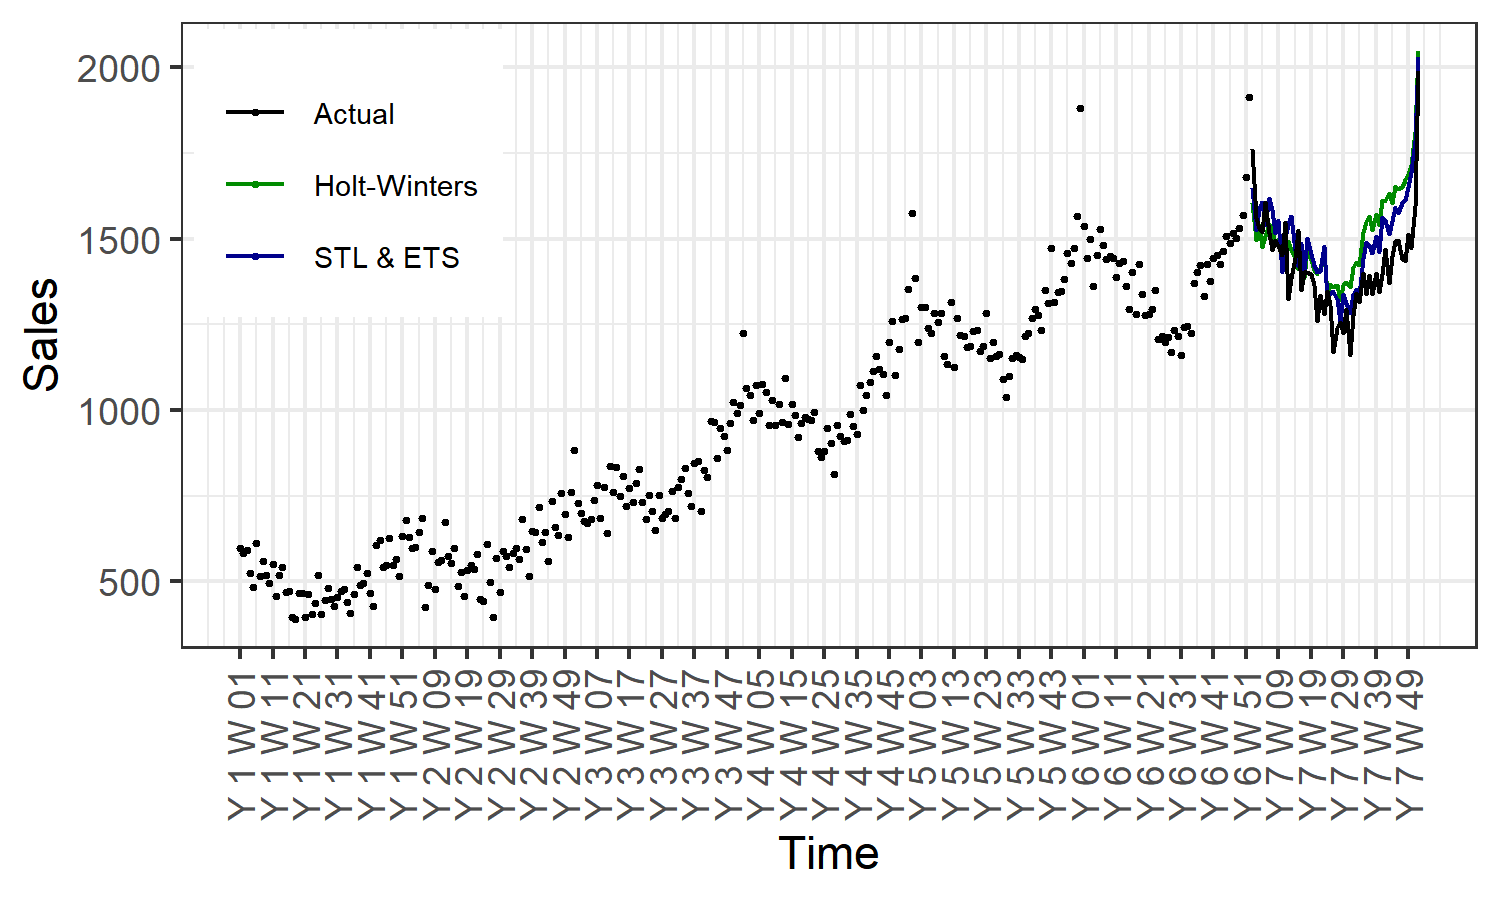
\includegraphics[width = 0.9\textwidth]{"figures/hw_stl.png"}
\caption{Comparison between forecasts from Holt-Winters and STL decomposition combined with exponential smoothing for the trend.}
\label{fig:hw_stl}
\end{figure}

In the ARIMA(p,d,q)(P,D,Q) method, each observation of the stationary series is taken as a linear combination of the past observations in an autoregressive model, and of the past error terms with a moving average. The ARIMA method requires stationary time series. In practice we obtain this applying differencing. The first order of differencing (d = 1) gives the differenced time series $y_t = F_t - F_{t-1}$. Similarly for a periodic system with $m$ the length of the period the seasonally differenced time series of first order ($D = 1$) is given by $y_t = F_t - F_{t-m}$. The moving average component has the form: 
\begin{equation}
y^{d,q}_t = \mu + \epsilon_t + \theta_1 \epsilon_{t-1} + ... + \theta_q \epsilon_{t-q}, ~~~~~~~~~~|\theta_i|<1 ~~ i\in\{1, ..,q\},
\label{eq:moving_average}
\end{equation}
where $\epsilon_t$ is the error term. The target variable is expressed as the mean $\mu$ corrected with a linear combination of the errors of the previous $q$ terms. The autoregressive part is given by the equation, 
\begin{equation}
y^{d,p}_t = \epsilon_t + \phi_1 y_{t-1} + ... + \phi_p y_{t-p}, ~~~~~~~~~~|\phi_i|<1 ~~ i\in\{1, ..,p\},
\label{eq:autoregression}
\end{equation}
where the target value is given in terms of previous target values. Iterating for $p = 1$, eq.\ref{eq:autoregression} can be expressed in terms of all past error terms as $y^{d,p}_t = \sum_{k= 0}^{t-1}\phi_1^k\epsilon_{t-k}+\phi_1^t y_0$. Since $\phi_1$ is smaller than one, the higher the power of $\phi_1$, the smaller the contribution of past error terms will be. For $p=1$, the main contribution to the target value is given by the recent error terms $\epsilon_t$ and  $\epsilon_{t-1}$. In the usual regression methods the target values are given by a function that depends on time in an explicit way. In autoregressive techniques, the target values are given by a linear combination of the recent target values and do not depend explicitly on time. For this type of models the causality is an intrinsic property of the mechanism. Moreover the more recent target values contribute with higher weights (given by the power of the regression coefficients), while distant contributions are negligible. This can be seen as a local mechanism, because only the recent target values influence directly the value of the prediction. Similarly to eq.\ref{eq:moving_average} and eq.\ref{eq:autoregression} one can construct the equations for the seasonal components $Q$ and $P$ respectively taking contributions from recent target values in distance equal to the length of a seasonal period. Such distant values will contribute with higher weights to the seasonal ARIMA than the would contribute to the non-seasonal. Therefore one may include the different terms in a general form of an ARIMA equation which takes the form
\begin{equation}
y^{(p,d,q)(P,D,Q)}_t = y^{D,d,p}_t +  y^{D,d,q}_t +  y^{D,d,P}_t +  y^{D,d,Q}_t + R_t,
\end{equation}
where $R_t$ stands for any other regression variables taken into account in the model. 

\begin{figure}[h!]
\centering
\begin{subfigure}{0.7\textwidth}
\caption{Seasonal differencing}
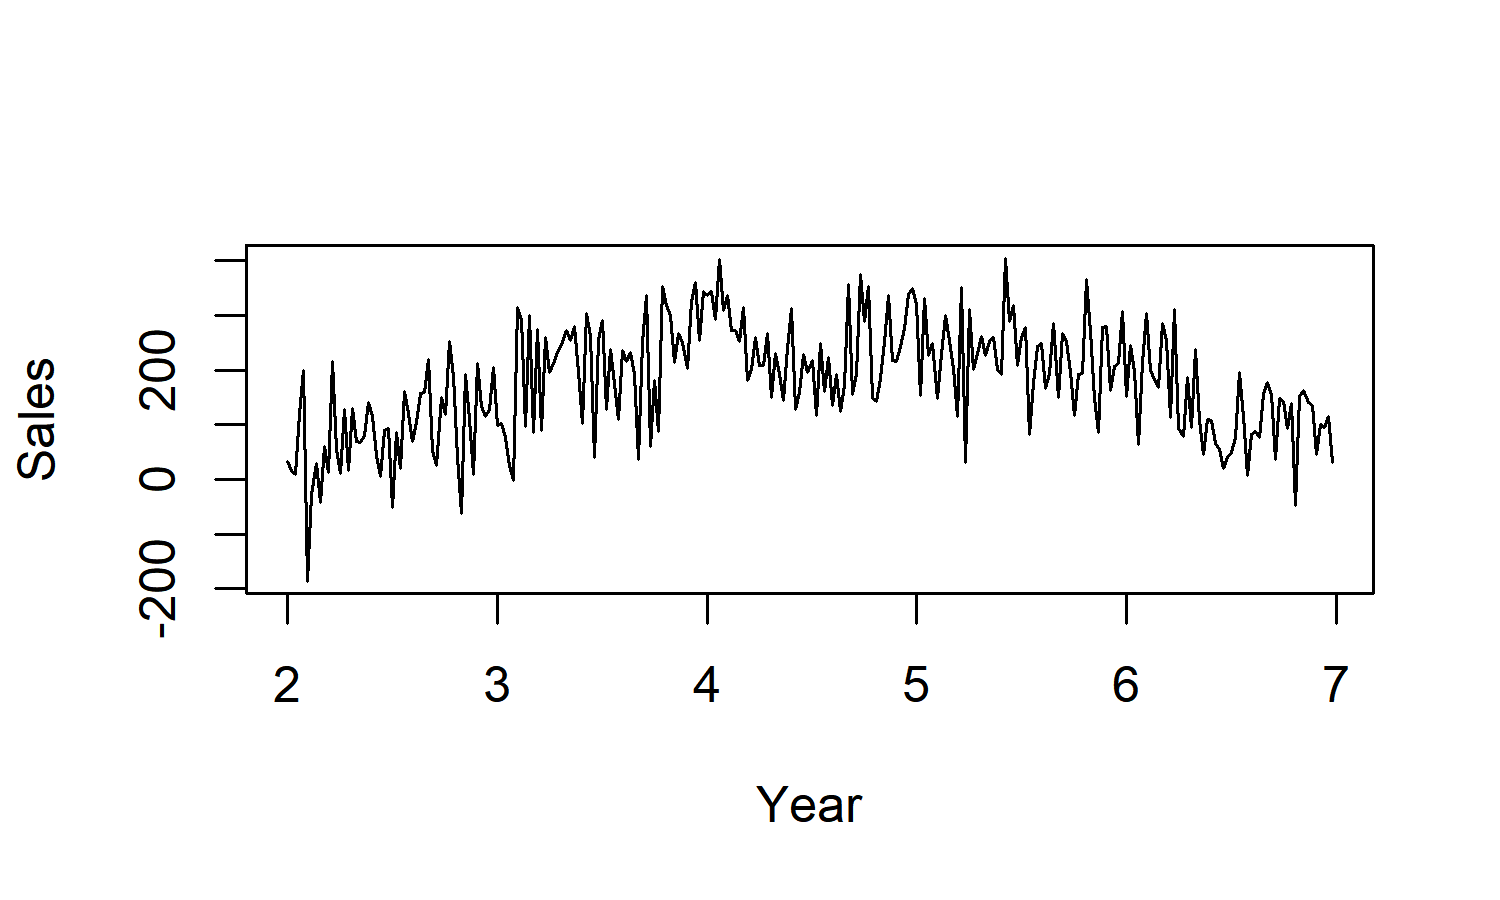
\includegraphics[trim = {0 1.5cm 0 2cm}, clip, width = \textwidth]{"figures/ts.png"}
\label{fig:seasdiff}
\end{subfigure}
\vfill
\begin{subfigure}{0.7\textwidth}
\caption{Non-seasonal differencing}
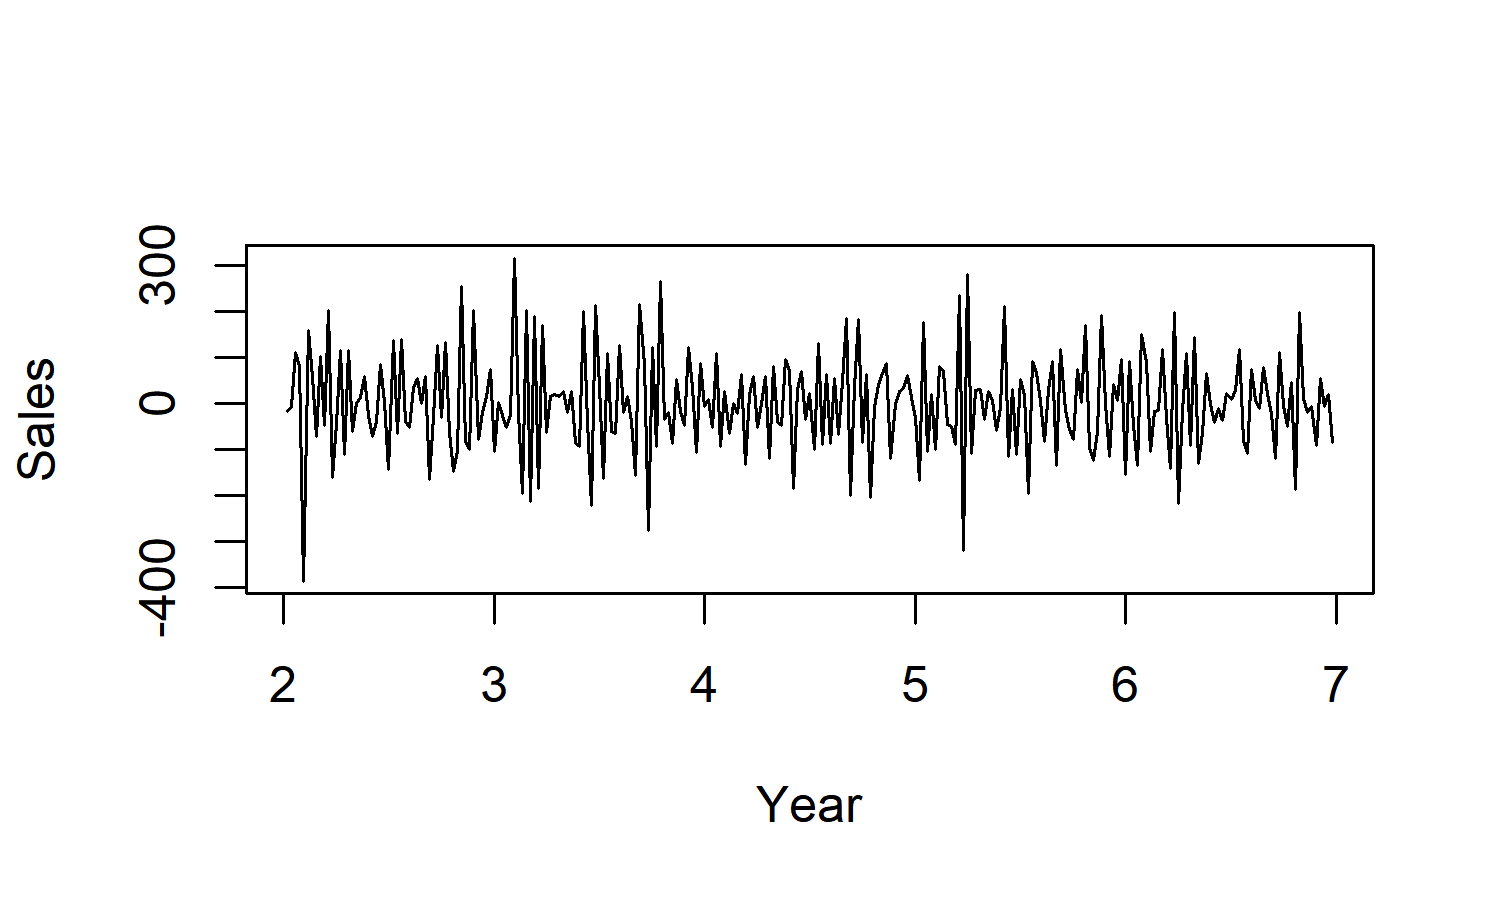
\includegraphics[trim = {0 0.5cm 0 2cm}, clip, width = \textwidth]{"figures/ts1.png"}
\label{fig:nseasdiff}
\end{subfigure}
\caption{Differenced timeseries.}
\label{fig:differencing}
\end{figure}

\begin{figure}[h!]
\centering
\begin{subfigure}{0.49\textwidth}
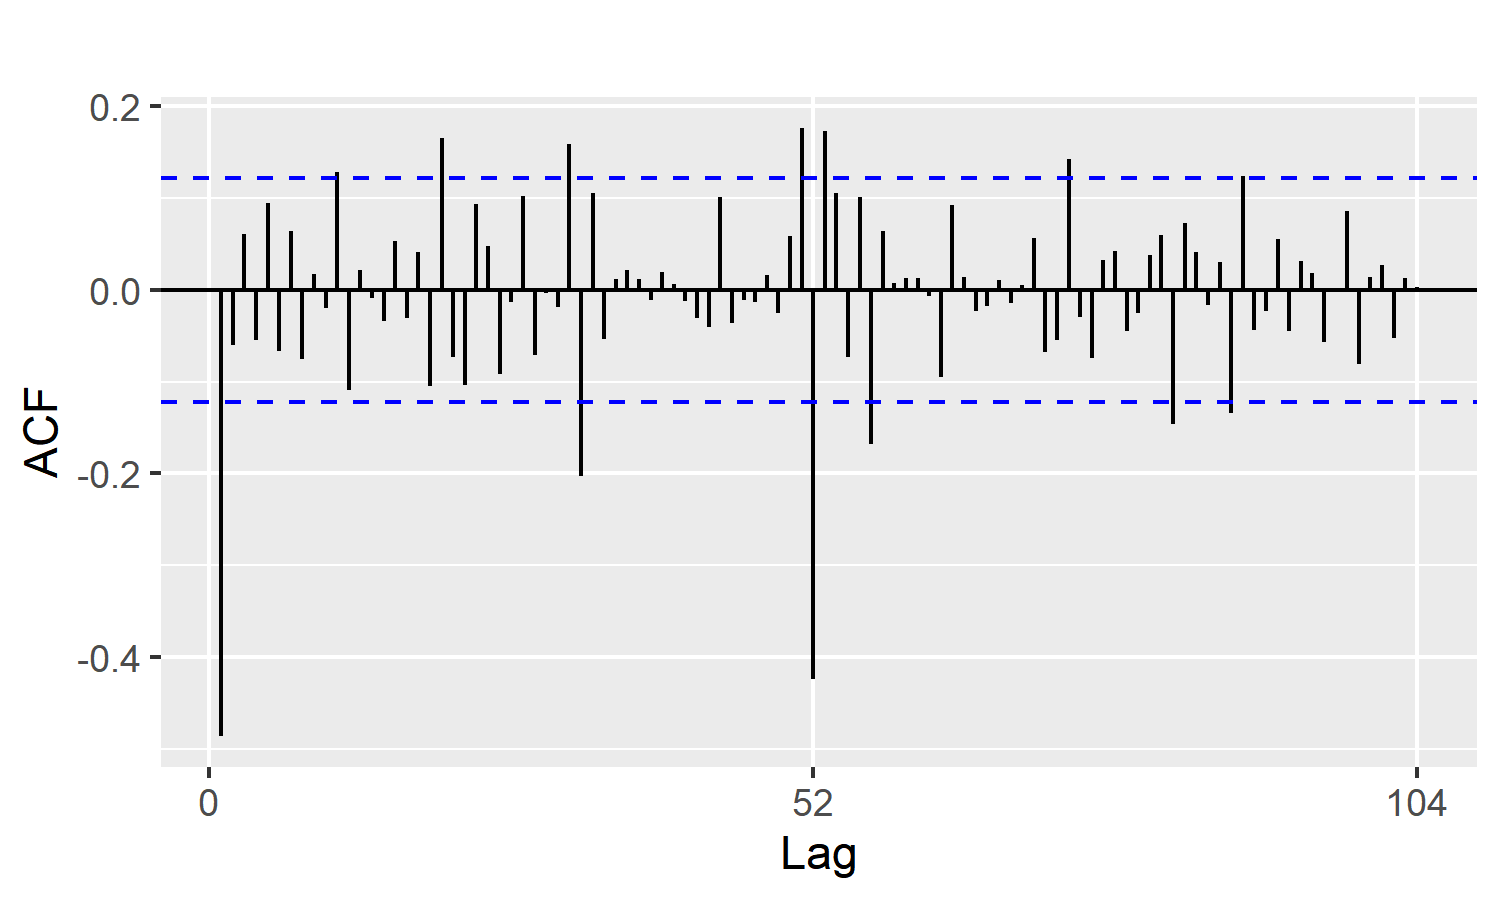
\includegraphics[width = \textwidth]{"figures/ACF.png"}
\caption{Autocorrelation}
\label{fig:ACF}
\end{subfigure}
\hfill
\begin{subfigure}{0.49\textwidth}
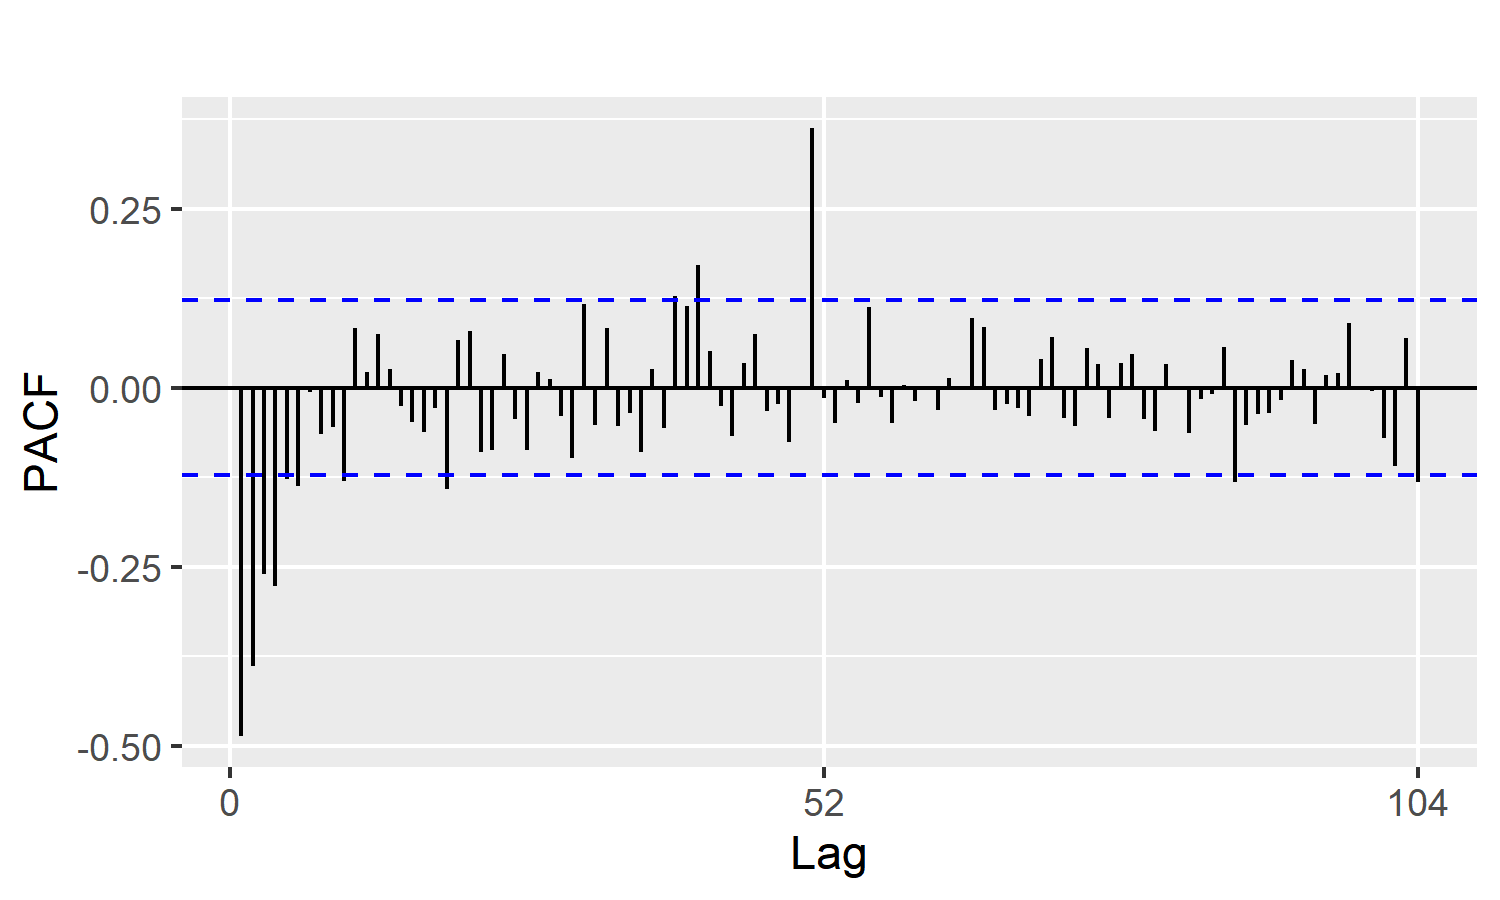
\includegraphics[width = \textwidth]{"figures/PACF.png"}
\caption{Partial autocorrelation}
\label{fig:PACF}
\end{subfigure}
\caption{Correlation as a function of the lag.}
\label{fig:correlation}
\end{figure}

In fig.\ref{fig:differencing} applying first seasonal differencing on the time series (D = 1) and then simple differencing (d = 1) results in stationary time series. This in practice is verified using a KPSS test \cite{KPSS}. Fig.\ref{fig:correlation} shows the plots of the autocorrelation (ACF) and partial autocorrelation (PACF) functions for this data set. The strong first peak of the ACF plot suggests that the first order is significant for the moving average part. The first 4 strong peaks of the PACF plot suggest that four terms play a role in the autoregressive part. A peak at lag 52 of the ACF and  PACF plots indicate the first order as possible candidate for the moving average or autoregressive terms of the seasonal part. In practice the orders of the autoregression and of the moving average can be calculated using the maximization of an information criterion, or minimization of the cross-validation error. Using the maximization of the Akaike's Information Criterion (AIC) in the implementation of Hyndman and Khandakar \cite{autoarima} the resulting model is the ARIMA(0,1,2)(1,1,1). On the other hand, the model ARIMA(1,1,1)(1,1,1) is minimizing the cross-validation error. For the cross-validation we used a step of 10 weeks for expanding the training window instead of 1 week and distributed the iteration over the values of the order parameter to 8 logical processors. Introducing $\frac{1}{Price}$ as an additional variable, the resulting model from ARIMA with AIC is the ARIMA(0,1,1)(1,1,1). We evaluated the order parameters using the full data set. Then we obtain the autoregression and moving average coefficients from fitting a training set and evaluate the prediction error. Finally we apply the final model on the full data set and calculate the forecast. 

In fig.\ref{fig:arima} we compare the forecast obtained from the information criterion (without price with the red line and with price with the orange line) with the forecast obtained from cross-validation (blue line). The forecast that includes the effect of the price is very similar to the forecast without price and the two lines are on top of each other. The order obtained with cross-validation gives a forecast that is slightly better. Comparing the errors in tab.\ref{tab:Comparison}, cross-validation slightly improves all errors. The ARIMA from AIC compared to the Holt-Winters improves the fitting, but slightly aggravates the prediction and cross-validation errors. Nevertheless the errors of the two methods, ARIMA and Holt-Winters, are close, so it makes sense to further examine the performance of both methods on a realistic data set. Including the price as a predictor in the ARIMA method (orange line) has a negligible effect to the performance of the model even though it reduces the order of the moving average term in the non-seasonal part of the method. 

\begin{figure}[h!]
\centering
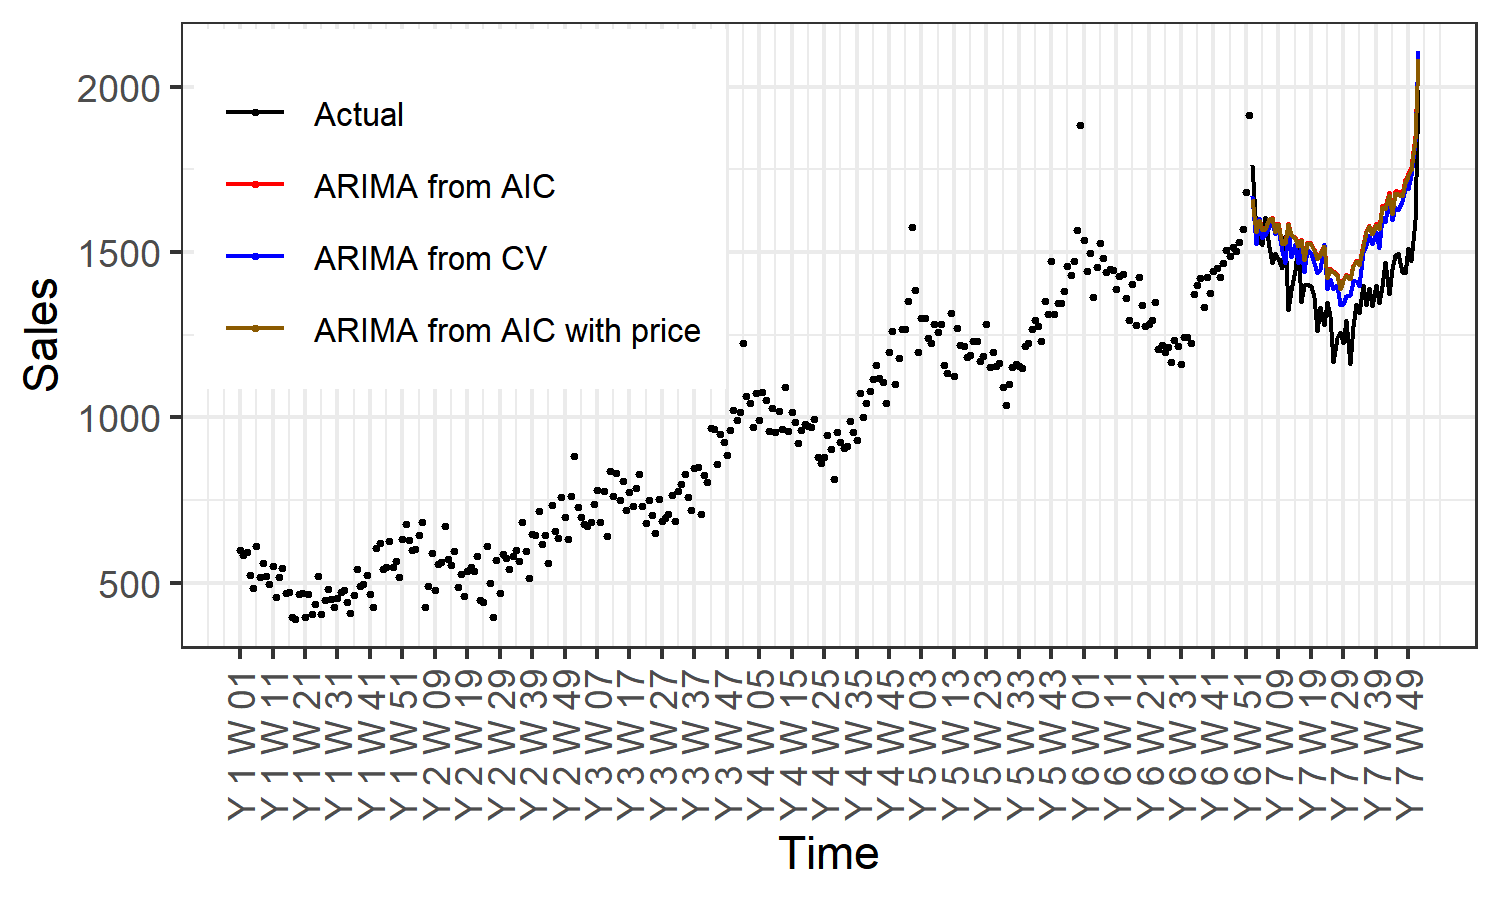
\includegraphics[width = 0.9\textwidth]{"figures/arima.png"}
\caption{Forecasting with the ARIMA method.}
\label{fig:arima}
\end{figure}

\newpage

\begin{table}[h!]
\begin{tabular}{ | m{3cm} | m{1.8cm}| m{1.8cm} | m{3cm} |m{2.5cm} |} 
\hline\vspace{0.1cm}
Method & Fitting & Prediction & Cross-validation & Decomposition\\ 
\hline\hline\vspace{0.1cm}
Seasonal naive & 216.34 & 148.06 & 197.74 & - \\
\hline\vspace{0.1cm}
Naive with drift & 83.09 & 638.74 & 175.35 & - \\
\hline\vspace{0.1cm}
Seasonal linear model & 57.01 & 99.3 & 116.37 &- \\ 
\hline\vspace{0.1cm}
CD - LR & 30.48 &  26.27 & 61.08 & 57.32\\ 
\hline\vspace{0.1cm}
CD - NLR & 5.57 & 14.57 & 28.96 & 57.32 \\
\hline\vspace{0.1cm}
CD - Ss & 4.14 & 56.58 & \textcolor{red}{32.82} & 57.32 \\
\hline\vspace{0.1cm}
STL \& naive & 71.68 & 77.99 & 133.22 & 49.74\\
\hline\vspace{0.1cm}
STL \& drift & 71.61 & 93.06 & 96.93 & 49.74\\
\hline\vspace{0.1cm}
STL \& ETS & 52.22 & 106.42 & 97.86 & 49.74\\
\hline\vspace{0.1cm}
STL - NLR & 6.84 & 30.69 & \textcolor{red}{29.8} & 49.74\\
\hline\vspace{0.1cm}
Holt-Winters & 73.1 & 130.66 & \textcolor{red}{90.2} & - \\
\hline\vspace{0.1cm}
ARIMA from AIC & 61.47 & 166.81 & \textcolor{red}{95.4 (step = 1) / 98.35 (step = 10)}& - \\
\hline\vspace{0.1cm}
ARIMA from CV &  54.37 & 162.41 & \textcolor{red}{86.11 (step = 10)} & - \\
\hline\vspace{0.1cm}
ARIMA from AIC with price & 61.05 & 179.07 & \textcolor{red}{96.83 (step = 1)}& - \\
\hline
\end{tabular}
\caption{Comparison of the performance of different methods. With red color we emphasize the cases that suggest improvements and can be applied further in a realistic case.}
\label{tab:Comparison}
\end{table}

\newpage

\subsection{A note on the computational performance}
In the artificial data set we could already sense that the cross-validation process for selecting the order of a more complex method like the ARIMA is computationally expensive and it took approximately 20 minutes to run. For that calculation we even reduced the size of the cross-validation set, by using a step of 10 weeks for the expanding window of the training set, instead of 1 week. So it can be expected that applying this method to obtain several forecasts or trying to make it more precise will further increase the computational cost.

In all the methods the most computationally expensive part is the cross-validation process. For simpler models like the Holt-Winters where the model parameters are defined on the training set, the cross-validation performs iterations only over the train-test subsets. To speed up that part we distributed to 8 processors the fitting of the models for the different subsets of the cross-validation. It takes approximately 10 minutes to run the cross-validation in this setup for a 100 of time series. For the regression with polynomials and smoothing splines, it is not only the iteration over the subsets in the cross-validation, but also the iteration over the model hyperparameters that increases the computational cost. For these models we distributed the iteration over the model hyperparameters and computed the cross-validation errors in a sequential manner, in order to avoid distributing the cross-validation in each iteration of the hyperparameters which could increase the overhead. For the polynomials it takes around half an hour to obtain a 100 forecasts, while for the smoothing splines it takes a couple of hours. The computational time also depends on the complexity of the model that we try to fit as well as the number of the hyperparameters we include and the size of the grid of values we are searching. The ARIMA process with the order selection with AIC is the most computationally expensive model that we attempted to apply in the realistic data set so far. Therefore we tried two different approaches. The first involves to distribute the order selection and cross-validation processes for each of the different objects in the data set. The second involves the distribution of the data set over multiple processors and to run the fitting and cross-validation processes in a sequential manner. We compared the performance of the two approaches only for a subset with 10 time series and the first approach still runs faster. It would be interesting to make the same comparison for the full data set increasing the computational power, and see if there is a limit where distributing the data set instead of the tasks becomes more efficient.

\section{Conclusions and recommendations}

Starting from an artificial data set we studied the performance of different methods for sales forecasting. On one hand we decomposed the time series to its seasonal and trend components and obtained forecasts for the trend while repeating the seasonal behavior of the last year of observations. On the other hand, we calculated forecasts for both the seasonal and trend components based on the past observations. We applied the most promising methods on a realistic data set and discussed their performance. 

The regression for the trend is modeling the explicit behavior of the target variable as a function of time. This has the drawback that causality is not taken into account in the model, and other time series properties are taken into account only through the adaptation of the cross-validation process to perform forward predictions which is used for estimating the hyperparameters of the model. On the contrary the ARIMA and Holt-Winters' methods do not depend on time, but rather on the values of the target variable in the recent past which explicitly accounts for causal effects. Moreover polynomials and smoothing splines suffer from deviations outside of the fitting region, and since we can only use information from the past to determine the forecasts (absence of an upper boundary), they can give forecasts with unrealistic deviations. On the contrary the ARIMA and Holt-Winters' methods effectively attribute smaller weights to the distant-past observations so that they have a smoothing effect on the values predicted from the recent terms. In overall the advantages presented by the Holt-Winters and ARIMA methods outweigh the performance of the regression methods. Holt-Winters is relatively easier and faster to perform and in most of the cases it performs as well as ARIMA. On the contrary ARIMA is a more flexible method which leads to more reliable forecasts but it is computationally expensive. In overall the Holt-Winters method offers a good balance between performance, computational cost and interpretability and can be used to benchmark against further improvements or more complex approaches than the ones that we discussed here.

The main challenge on a realistic data set is to model and forecast all the time series following a single approach. In order to further optimize the performance of the single methods one could look for a hybrid approach. For example one can start with a generally well-performing model like the Holt-Winters' method and calculate the errors. For cases where all the cross-validation and prediction errors are large (e.g. larger than a standard deviation) one can try to apply a more complex method like the ARIMA. In general it is not clear whether including predictors like the price or the inverse price in the ARIMA method will lead to significant improvements. But in order to capture a non-trivial dependence on a predictor (like the one in the artificial data set), one can use cross-validation to try different non-linear models, and include such predictors in the ARIMA method. 

Until now we have been looking for patterns in each individual object separately. However often the sales of the same product from different places can show similar patterns. Also products that belong in the same product-category can show similar characteristics. It is possible to evaluate the model hyperparameters, like the order of an ARIMA model or a smoothing parameter, on a product category and use them to build the single-object models for all products that belong to that category in order to obtain the forecasts. This is a way to not only speed up the model selection of the ARIMA process, but also impose the additional constraint that all products in the same category should follow a similar mechanism. It would be interesting to see how reliable such forecasts are compared to modeling each individual object separately. Also the default categorization of products in the data set does not always succeed to describe the characteristics of all the products that fall under a given category. In order to achieve a better categorization as well as distinguish the products that do not fall under any category, one could apply clustering techniques grouping together similar time series vectors. Finally, another approach that would be interesting to try, is to model and forecast a product category with a reliable method i.e. the ARIMA, and then use such a forecast as an additional predictor variable in order to determine the forecast of the single objects. 

\begin{thebibliography}{9}
\bibitem{Hyndman_book} 
Hyndman, R.J., \& Athanasopoulos, G. (2018) 
\textit{Forecasting: principles and practice, 2nd edition, OTexts: Melbourne, Australia.} 
\\\texttt{OTexts.com/fpp2}. 
Accessed on 21/04/2021 

\bibitem{STL}
Cleveland, R. B., Cleveland, W. S., McRae, J. E., \& Terpenning, I. J. (1990) 
\textit{STL: A seasonal-trend decomposition procedure based on loess.} 
Journal of Official Statistics, 6(1), 3–33. 
\\\texttt{http://bit.ly/stl1990}

\bibitem{Winters}
Peter R. Winters (1960)
\textit{Forecasting Sales by Exponentially Weighted Moving Averages.} 
Management Science 6 (3) 324-342 
\texttt{https://doi.org/10.1287/mnsc.6.3.324}

\bibitem{Holt}
C. C. Holt (1957)
\textit{Forecasting seasonals and trends by exponentially weighted moving averages.} 
ONR Research Memorandum, Carnegie Institute of Technology 52 
\texttt{reprint at https://doi.org/10.1016/j.ijforecast.2003.09.015}
 
\bibitem{ARIMA}
Box, G. E. P., Jenkins, G. M., and Reinsel, G. C. (1994) 
\textit{Time Series Analysis, Forecasting and Control, 3rd ed.} 
Prentice Hall, Englewood Clifs, NJ.

\bibitem{autoarima}
Hyndman, R. J., \& Khandakar, Y. (2008) 
\textit{Automatic time series forecasting: The forecast package for R.} 
Journal of Statistical Software, 27(1), 1–22. 
\texttt{https://doi.org/10.18637/jss.v027.i03}

\bibitem{KPSS}
Kwiatkowski D, Phillips PCB, Schmidt P and Shin Y (1992) 
\textit{Testing the Null Hypothesis of Stationarity against the Alternative of a Unit Root.} 
Journal of Econometrics 54:159-178.

\bibitem{Statistical_Learning}
Gareth James, Daniela Witten, Trevor Hastie, Robert Tibshirani. 
\textit{An Introduction to Statistical Learning : with Applications in R.}
New York :Springer, 2013.

\bibitem{Smoothing_Splines}
Wood, S.N. (2003) 
\textit{Thin plate regression splines.} 
J.R.Statist.Soc.B 65(1):95-114

\end{thebibliography}

\end{document}


